\documentclass[4pt]{article}
\usepackage{pdflscape}
\usepackage[margin=0.2in,top=0.1in,bottom=0.1in]{geometry}
\usepackage{multicol}
\usepackage{parskip}
\usepackage{titlesec}
\usepackage{xcolor}
\titlespacing*{\subsubsection}{0pt}{10pt}{*0}

\usepackage{amsmath}
\usepackage{amssymb}
\usepackage{amsthm}
\usepackage{siunitx}
\usepackage{esint}
\usepackage{hanging}
\usepackage{xfrac}
\usepackage{tikz}
\usetikzlibrary{positioning}
\pagenumbering{gobble}

\theoremstyle{definition}
\newtheorem*{claim}{Claim}
\theoremstyle{definition}
\newtheorem*{lemma}{Lemma}
\renewcommand{\qed}{\hfill\blacksquare}
\renewcommand{\c}{\mathrm{c}\,}
\newcommand{\s}{\mathrm{s}\,}
\renewcommand{\r}{\mathrm{r}\,}             % abbreviation for rect()
\renewcommand{\o}{\omega}
\newcommand{\ra}{\rightarrow}
\newcommand{\lra}{\leftrightarrow}
\newcommand{\ulint}{\int_{0^-}^{\infty}}    % Unilateral Lt INTegral
\DeclareMathOperator{\rect}{rect}
\DeclareMathOperator{\sinc}{sinc}
\DeclareMathOperator{\sgn}{sgn}
\newcommand{\red}[1]{\textcolor{red}{#1}}
\newcommand{\blue}[1]{\textcolor{blue}{#1}}

\newcolumntype{Y}{>{\centering\arraybackslash}X}
\setlength{\abovedisplayskip}{0pt} % Space above display math
\setlength{\belowdisplayskip}{0pt} % Space below display math
\setlength{\abovedisplayshortskip}{0pt} % Space above when preceded by a short line
\setlength{\belowdisplayshortskip}{0pt} % Space below when followed by a short line


\title{Signals and Systems Exam 3}
\usepackage{fancyhdr} % For custom headers and footers

\begin{document}
\begin{landscape}
\raggedright
\begin{multicols}{3} % Use 3 columns
\raggedcolumns
%\section*{Foundation}
\subsubsection*{\blue{Algebra}}
    $\sin n\pi = 0$\\
    $1-\cos n\pi = 2$ for odd $n$\\
    $\arctan(\frac{1}{\sqrt{3}}) = \frac{\pi}{6}$,  $\arctan(\sqrt{3}) = \frac{\pi} 3$

    $\sin(x\pm y) = \sin x \cos y \pm \cos x \sin y$\\
    $\cos(x\pm y) = \cos x \cos y \mp \sin x \sin y$

    $\sin x \sin y = \frac{1}{2}[\cos(x-y) - \cos(x+y)]$\\ % annotate for sin 2x and cos 2x
    $\cos x \cos y = \frac{1}{2}[\cos(x-y) + \cos(x+y)]$\\
    $\sin x \cos y = \frac{1}{2}[\sin(x-y) + \sin(x+y)]$

    \(\sin a \pm \sin b = 2\sin \frac{a+b}{2} \cos \frac{a\mp b}{2}\)\\
    \(\cos a + \cos b = 2\cos \frac{a+b}{2} \cos \frac{a-b}{2}\)\\
    \(\cos a - \cos b = -2\sin \frac{a+b}{2} \sin \frac{a-b}{2}\)

    $C \cos(\o_0 t + \theta) = C\cos(\theta) \cos(\o_0 t) \red - C\sin(\theta)\sin(\o_0 t)$\\ 
    $C \sin(\o_0 t + \theta) = C\sin(\theta) \cos(\o_0 t) + C\cos(\theta)\sin(\o_0 t)$

    $\theta = \tan^{-1} (\red - \frac b a)$, $\pm \pi$ when $a<0$\\
    $\sin t = \cos (t - \frac{\pi}{2})$\\
    \(-\cos t = \sin(t - \frac{\pi}{2})\)

    $\cos x = \frac{1}{2}\,[e^{jx} + e^{-jx}]$\\
    $\sin x = \frac{1}{2 \red j}\, [e^{jx} - e^{-jx}]$\\
    $e^{j\o t} = \cos(\o t) + j\sin (\o t)$

    $z^* = a-jb = re^{-j\theta}$\\
    $u^* v^* = (uv)^*$

    $\angle z = \tan^{-1}(\frac b a)$, $\pm \pi$ in Q2 and Q3

    $z^{\frac 1 n} = r^{\frac 1 n} e^{j \frac{\theta + 2\pi m}{n}}$

    \((s+a)(s+b)(s+c) = s^3 + (a+b+c) s^2 + (ab+bc+ca)s + abc\)
%\rule{\linewidth}{0.5pt}
\subsubsection*{\blue{Integrals}}

    $\int \cos^2 at \, dt = \frac{t}{2} + \frac{\sin2at}{4a}$

    $\int t \cos at \, dt = \frac{1}{a^2}(\cos at + at\sin at)$\\
    $\int t \sin at \, dt = \frac{1}{a^2}(\sin at - at\cos at)$\\
    $\int t^2 \cos at\, dt = \frac{1}{a^3}(2at\cos at - 2\sin at + a^2t^2\sin at)$\\
    $\int t^2 \sin at\, dt = \frac{1}{a^3}(2at\sin at + 2\cos at - a^2t^2\cos at)$

    $\int te^{at}\, dt = \frac{1}{a^2} \, e^{at} (at-1)$\\
    $\int t^2 e^{at} \, dt = \frac{1}{a^3} \, e^{at} (a^2t^2 - 2at + 2)$

    $\int e^{at} \,\cos bt \, dt = \frac{1}{a^2+b^2} \,e^{at}(a\cos bt + b \sin bt)$\\
    $\int e^{at} \,\sin bt \, dt = \frac{1}{a^2+b^2} \,e^{at}(a\sin bt - b \cos bt)$

    \(\int \frac{1} {x^2+a^2}\, dx = \frac{1}{a} \tan^{-1} \frac x a\)
\columnbreak
\subsubsection*{\blue{Signals}}
    $\mathcal{E}_f = \int_{-\infty}^{\infty} |f(t)|^2 dt$ (complex); \\
    $P_f = \lim_{T\ra\infty}\frac{1}{T} \int^{T/2}_{-T/2} |f(t)|^2 dt $; \\
        \hspace{1em} rms power $= \sqrt {P_f}$

    % can't be both energy/power
    Cont; 
    analog; 
    periodic (extension); 
    (non/anti)causal; 
    energy/power (both); 
    deterministic/stochastic (info)

    $\int f(t) \cdot \delta(t - t_0) dt = f(t_0)$ ($f$ continuous at $t_0$)
    

    $f(2x-6)$: shift by 6, scale by 2;\\
    $f(2(x-6))$: scale by 2, shift by 6

    $f_e(t) = \frac{1}{2}[f(t) + f(-t)]$\\
    $f_o(t) = \frac{1}{2}[f(t) - f(-t)]$
\subsubsection*{\blue{Systems}}
    % not all systems are like that, note
    $\mathcal{T}$: $\sum_{k=0}a_k D^k \, y(t) = \sum_{l=0}b_lD^l\, f(t)$

    \blue{Linear} $\mathcal{T}[kf_1(t) + f_2(t)] = ky_1(t) + y_2(t)$.\\
        \hspace{1em} Lin if $a_k$, $b_l$ are not functions of $y(t), f(t)$\\
            \hspace{2em} E. $\sin\dot{y}(t) + t^2 y(t) = (t+3) f(t)$
    
    \blue{Time-inv} $\mathcal{T}[f(t-\tau)] = y(t-\tau)$.\\
        \hspace{1em} $a_k$, $b_l$ indep of $t$ (const coeff)\\
        \hspace{1em} Let $g(t)\equiv f(t-\tau)$, find $z(t) = \mathcal{T}[g(t)]$, cmp $y(t-\tau)$


    \blue{Causal} $y(t)$ dep only on $f(\tau)$, $\tau \leq t$. 
    Compare $t$ and $\tau$.
    
    \blue{Instantaneous} $y$ only dep $f$ at present (no $\int$, no memory)
    
    \blue{Invertible} given $y(t)$, we can know $f(t)$ (ideal diff is not)
\subsubsection*{\blue{Conv prop}}
    $c(t) \equiv \int_{-\infty}^{\infty} f(\tau) g(t-\tau) \, d\tau$\\
    \(c[n] \equiv \sum_{m = -\infty}^{\infty} f[m] g[n-m]\)          % textbook p587


    $f * g = g * f$\\
    $f * (g + h) = f * h + g * h$\\
    $f * (g * h) = (f * g) * h$\\
        \hspace{1em} pf: $f * (g * h) = f * (h * g)$\\
            \hspace{2em} \(= \int f(\tau_1) \int h(\tau_2)\, g(t - \tau_2 - \tau_1) \, d\tau_2 \, d\tau_1\)\\
            \hspace{2em} \(= \int h(\tau_2) \int f(\tau_1)\, g(t - \tau_1 - \tau_2) \, d\tau_1 \, d\tau_2\)
    
     $f(t - T_1) * g(t - T_2) = c(t - T_1 - T_2)$

     $f(at) * g(at) = |\frac{1}{a}|\, c(at)$ (even/odd)

     $f^{(m)} (t) * g^{(n)} (t) = c^{(m+n)}(t)$\\
        \hspace{1em} pf: \(\dot f(\tau) = \lim_{T\ra 0} f(\tau) - f(\tau - T)\)


    Graph: shift \red{left} by $\red + t$, and reflect;\\
        \hspace{1em} Every $\tau$ replaced by \red{$t-\tau$}; Reverted
\columnbreak
\subsubsection*{\blue{Conv table}}
    $f(t) * \delta(t-T) = f(t-T)$
    
    $u(t) * u(t) = t \, u(t)$

    $e^{at} \,u(t)* \,u(t) = \frac{1-e^{at}}{-a}\, u(t)$

    % Watch the sign.
    $e^{\red{a}t}\,u(t) * e^{\red{b}t}\,u(t) = \frac{e^{at} - e^{bt}}{a - b}\, u(t)$        \hfill $a=b$, $te^{at} \, u(t)$ 

    $e^{at}\, u(t) * e^{bt} \, u(\red{-}t) = \frac{e^{at} \, u(t) + e^{bt} \, u(-t)}{b-a}$  \hfill $\Re(b) > \Re(a)$

    % + here
    $te^{at}\,u(t) * e^{at} \,u(t)= \frac{1}{2} \,t^2e^{at} \, u(t)$

    $t^m\, u(t) * t^n \, u(t) = \frac{m!\, n!}{(m+n+1)!}\, t^{m+n+1} \, u(t)$

    Don't forget $[u(t+T_1) - u(t-T_2)]$ term       % global highlight
\subsubsection*{\blue{LTI response}}
    $Q(D) y(t) = P(D) f(t)$, typically integrating $f$\\
    Assume causal input $f(t) u(t)$

    $y_{\blue{zs}}(t) = f(t) * h(t)$ from input\\    
        $y_{zs}(0^-) = 0$, $y_{zs}(0^+) \neq 0$

        % textbook p120
        Let $h(t) = \mathcal{T} [\delta (t)]$ (impulse response)\\
        % More description here
            \hspace{1em} $y_{zs}(t)=\mathcal{T} [f(t)] = \mathcal{T} [f(t) * \delta (t)]$\\
                \hspace{2em} $=\mathcal{T}[\lim\sum f(n\Delta\tau) \delta(t - n\Delta\tau) \Delta\tau]$\\
                \hspace{2em} $=\lim\sum f(\blue{n\Delta\tau}) h(t - \blue{n\Delta\tau}) \blue{\Delta\tau} = f * h$
            % linearity allows sum manipulation
            % time-invariance allows converting from \delta to h
            % sum turned to integral
            
        $y_{\blue{zi}}(t)$ from ini, $f(t)=0$,
            $Q y_{zi}(t) = 0$\\
            % same for the derivatives of y
            $y_{zi}(0^-) = y_{zi}(0^+)$, $\dot{y_{zi}}(0^-) = \dot{y_{zi}}(0^+)$
%\section{FS}
\subsubsection*{\blue{Ortho set}}
    $\mathcal{E}_e = \int_{t_1}^{t_2} [e(t)]^2 dt$\\
        $= \int_{t_1}^{t_2} f^2(t)dt - 2\sum c_i \int_{t_1}^{t_2} f(t) x_i(t) dt + \int_{t_1}^{t_2} (\sum c_i x_i(t))^2 dt$\\
        \hspace{1em}$= \mathcal{E}_f -  2\sum_{c_i} \langle f, x_i \rangle$\\
            \hspace{2em}$+(\sum c_i^2 \int_{t_1}^{t_2} x_i(t)^2 dt + \sum_{i\neq j} c_i c_j \int_{t_1}^{t_2} x_i(t) x_j(t) dt)$
        
    $\frac{\partial \mathcal{E}_e}{\partial c_i} = 0 = -2 \langle f(t), x_i(t)\rangle + 2\mathcal{E}_i c_i$\\
    $\mathcal{E}_e^{\text{min}} = \mathcal{E}_f - \sum_{i=1}^N c_i^2 \mathcal{E}_i$

    \(c_i = \frac{1}{\mathcal{E}_i}\langle f, x_i\rangle = \frac{\int f(t) x(t) dt}{\int x_i^2(t) dt}\)    

    For ortho, $E_z = E_x + E_y$
        

    $|u+v|^2 = |u|^2 + |v|^2 + u^*v + v^*u$

    $\langle x(t), y(t)\rangle = \int_{t_1}^{t_2} x(t) y(t)^{\red *} \, dt = \int_{t_1}^{t_2} x(t) y(t) dt$ if real\\
    Use prod $\ra$ sum identities
\newpage
\subsubsection*{\blue{FS}}
%\vfill\null
%\columnbreak 
    $\red{a_0} = \frac{1}{T_0} \int_{T_0} f(t)\, dt$\\
    $\blue{a_n} = \frac{\red 2}{T_0} \int_{\red{T_0}} f(t) \cos(n\o_0t)\,dt$\\
    $\blue{b_n} = \frac{2}{T_0} \int_{T_0} f(t) \sin(n\o_0t)\,dt$\\
    Energy: $T_0$ for $n=0$; $T_0/2$ else
     
    \blue{Half wave sym} $f(t - \frac{T_0}{2}) = -f(t)$\\
    $a_{n_\mathrm{odd}} = \frac{4}{T_0}\int_{0}^{T_0/2} f(t) \cos (n\o_0 t) \, dt$

    $f(t) = \sum_{n=-\infty}^{\infty} F_n e^{jn\o_0 t}$\\
    $F_n = \frac{1}{T_0}\int_{T_0} f(t) e^{\red{-}jn\o_0t}\,dt$

    $C_n\cos(n\o_0 t + \theta_n) = \frac{C_n}{2} \, (e^{j(n\o_0t + \theta_n)} + e^{-j(n\o_0 t + \theta_n)})$\\
    $ \hspace{5em}= \blue{(\frac{C_n} 2 e^{j\theta_n})} e^{jn\o_0 t} + \blue{(\frac{C_n} 2 e^{\red{-}j\theta_n})} e^{-jn\o_0 t}$

    $F_n = \frac{C_n}{2}\, e^{j\theta_n} = \frac 1 2 (a_n \red{-} jb_n) = |F_n| e^{j\angle F_n}$\\
    $F_{-n} = \frac{C_n}{2}\, e^{-j\theta_n} = \frac 1 2 (a_n \red{+} jb_n)$ 
\subsubsection*{\blue{Existence}}
    Weak: finite $\int$, fin bounds $a$, $b$, fin power\\

    Strong: fin min/max/discont over $T_0$, $\ra \frac{f(t_0^+) + f(t_0^-)}{2}$
\subsubsection*{\blue{FS prop}}
    \blue{Time shift} $f(t-t_0)\ra F_n e^{-jn(\o_0 t_0)}$\\
        \hspace{1em} $|F_n|$ same; $\angle F_n$ shifted by $-(\o_0 t_0)n$

    \blue{Reversal} $f(-t)\ra F_{-n}$\\
    \blue{Scaling} $T = \frac {T_0} a$, $\o = a\o_0$

    \blue{Multiplication} (same $T_0$): $f(t) g(t) \ra F_n * G_n$\\ 
        \hspace{1em} $\frac 1{T_0}  \int_{T_0} f(t) g(t) e^{jn\o_0 t}\, dt$\\
        \hspace{1em} $ = \frac{1}{T_0} \int (\sum F_m e^{jm\o_0 t}) (\sum G_k e^{jk\o_0 t}) e^{-jn\o_0 t} \, dt$ \\
        \hspace{1em} $ = \sum_m \sum_k F_m G_k \frac{1}{T_0} \int_{T_0} e^{j(m+k-n)\o_0 t} \, dt$\\
        \hspace{1em} $ = \sum_m \sum_k F_m G_k \langle e^{j(m+k)\o_0 t}, e^{jn\o_0 t}\rangle$\\
        \hspace{1em} $ = \sum_{k=-\infty}^{\infty} G_k F_{n-k}$
        
    \blue{Conjugation} $f(t)^* = F^*_{-n}$

    \blue{Parseval} (power sig): \(P_f = \frac 1{T_0}\int_{T_0} f(t) f(t)^* dt\)\\
        \hspace{1em} \(=\frac{1}{T_0}\int_{T_0} (\sum_n F_n e^{jn\o_0t})(\sum_m F_m e^{jm\o_0t})^* dt\)\\
        \hspace{1em} \(=\sum_n \sum_m  F_n F_m^* \, \frac{1}{T_0}\int_{T_0} e^{j(n-m)\o_0t} dt\)\\
        \hspace{1em} \(=\sum_n |F_n|^2 \cdot 1\)

        $f$ real $\ra$ $|F|$ even, $\angle F$ odd\\
        $f$ real, even $\ra$ $F$ real, even; $F_{-n} = F_n = F_n^*$\\
        $f$ real, odd $\ra$ $F$ imaginary, odd; $-F_{-n} = F_n = -F_n^*$

        $f_e(t) \ra \Re\{ F_n\}$\\
        $f_o(t) \ra j \,\Im \{F_n\}$
\columnbreak
\subsubsection*{\blue{Common FS}}
    ($A=1$, $T=2\pi$, $\omega = 1$)\\
    \blue{Square}  
        $\frac{4}{\pi}(\cos t - \frac{1}{3}\cos 3t + \frac{1}{5} \cos 5t- ...)$\\
        $\frac{4}{\pi}(\sin t + \frac 1 3 \sin 3t + \frac 1 5 \sin 5t + ...)$

    \blue{Triangle} 
        $\frac{8}{\pi^2}(\sin t - \frac{1}{9} \sin 3t + \frac{1}{25} \sin 5t - ...)$\\
        $\frac{8}{\pi^2}(\cos t + \frac 1 9 \cos 3t + \frac 1 {25} \cos 5t + ...)$

    \blue{Sawtooth}   
        $\frac 2{\pi} (\sin t - \frac{1}{2} \sin 2t + \frac{1}{3} \sin 3t - ...)$\\
        $\frac 2{\pi} (-\sin t - \frac{1}{2} \sin 2t - \frac{1}{3} \sin 3t - ...)$

    \blue{$\delta$ train}    
        $\delta_{T_0} (t) = \sum_{n=-\infty}^{\infty} \delta(t - nT_0)$ \\
        $\frac{1}{T_0} \sum_{n=-\infty}^{\infty} e^{jn\omega_0 t}$

    % square duty cycle add here
%\section{FT}
\subsubsection*{\blue{FT}}
    Let \(F(\omega) \equiv \int f(t) e^{-j\omega t} \, dt\)

    \(F_n = \frac 1 {T_0} \int_{T_0} f(t) e^{-jn\omega_0 t} \, dt\)

    Limit as $\omega_0 =\Delta\omega \ra \blue 0$,\\
    \(F_n = \frac {\Delta\omega}{2\pi} \int_{\blue{-\infty}}^{\blue{\infty}} f(t) e^{-j \blue{n\Delta\omega} t} \, dt
    \equiv \frac{\Delta\omega}{2\pi} F(\blue{n\Delta\omega})\) % substitute t for n\Delta\omega

    \(f_{T_0}(t) = \sum F_n\, e^{jn\omega_0 t} = \sum \frac {\Delta\omega} {2\pi} F(n\Delta\omega)\,  e^{jn\Delta\omega t}\)

    % variable iof integration is \omega!
    % lim T0 -> infty
    % can also write delta \omega0/2pi = 1/T0
    % sum to integral
    \(f(t) = \lim_{T_0\ra \infty} f_{T_0} (t) = \red{\frac{1}{2\pi}}\int F(\omega) e^{jt\omega} d\omega\)

    \(F(\omega) = |F(\omega)| \, e^{j\angle F(\omega)}\)

    Real signals: amp and phase symmetry

    Existence: weak: energy signal ($|e^{-j\o t}| = 1$)\\
    Strong: fin num max/min/discont

\subsubsection*{\blue{FT Table}}

    \(\delta(t) \ra 1\)\\
    $1 \ra 2\pi\delta(\omega)$

    \(e^{j\o_0 t}\ra 2\pi\delta(\o \red{-} \o_0)\)\\         % inverse transform this
    \(\cos \o_0 t\ra \pi[\delta(\o+\o_0) + \delta(\o - \o_0)]\)\\
    \(\sin \o_0 t\ra \red{j}\pi[\delta(\o + \o_0) - \delta(\o - \o_0)]\)

    \(\sum \delta(t-nT_0) \ra \o_0\sum \delta(\o - n\o_0)\)             \hfill  $\o_0 = \frac{2\pi}{T_0}$

    $e^{-at} \, u(t) \ra \frac{1}{a+j\omega}$                           \hfill  $a > 0$\\
    $e^{-a|t|} \ra \frac{2a}{a^2+\omega^2}$                             \hfill $a > 0$\\
    \(u(t) = \lim_{a\ra 0} e^{-at} u(t)\ra \lim \frac{1}{a+j\o}\)\\
        \hspace{1em} \( = \lim(\frac{a}{a^2+\o^2} - j\frac{\o}{a^2+\o^2 }) = \pi\delta(\o) + \frac{1}{j\o}\) \\      % acrtan integral to get pi
    \(\sgn(t)\ra \frac{2}{j\o}\)

    \(t^n e^{-at} u(t)\ra \frac{n!}{(a+j\o)^{n+1}}\)                    \hfill $a > 0$
\columnbreak

    \(\cos \o_0 t\, u(t)\ra \frac{\pi}{2}(\delta(\o - \o_0) + \delta(\o + \o_0)) + \frac{j\o}{\o_0^2-\o^2}\)\\       
    \(\sin \o_0 t\, u(t)\ra \frac{\pi}{2\red{j}}(\delta(\o - \o_0) - \delta(\o + \o_0)) + \frac{\o_0}{\o_0^2-\o^2}\)\\
    \(e^{-at}\cos \o_0t\, u(t)\ra \frac{a+j\o}{(a+j\o)^2 + \o_0^2}\)    \hfill $a > 0$\\
    \(e^{-at}\sin \o_0t\, u(t)\ra \frac{\o_0}{(a+j\o)^2 + \o_0^2}\)     \hfill $a > 0$         


    % width \tau, draw a diagram
    $\rect(\frac t {\tau}) \ra \tau \sinc(\frac{\tau}{2}\omega)$\\ 
    $\frac W \pi \sinc(Wt) \ra \rect(\frac{\omega}{2W})$

    % draw a diagram as well
    \(\triangle (\frac t {\tau}) \ra \frac{\tau}{2} \sinc^2 (\frac{\tau}{4}\omega)\)\\
    \(\frac{W}{2\pi} \sinc^2 (\frac{W}{2}t) \ra \triangle(\frac{\omega}{2W})\)

    \([\o^2 \r(\frac{\o}{2\o_0})] \leftarrow \frac{1}{2\pi} \frac{e^{j\o t}}{(jt)^3}(-\o^2t^2-2j\o t + 2)^{\o_0}_{-\o_0}\)\\
    \(=\frac{(\o_0^2 t^2 - 2)\sin \o_0 t + 2\o_0 t\cos \o_0 t}{\pi t^3}\)\

    \([\frac{|\o|}{\o_0} \rect(\frac{\o}{2\o_0})] \leftarrow \frac{\cos \o_0 t + \o_0 t \sin \o_0 t - 1}{\o_0 \pi t^2}\)
\subsubsection*{\blue{Frequency domain prop}}
    \blue{Linearity}

    \blue{Time shift} \(f(t \red{-} t_0) \ra F(\omega) e^{\red{-} jt_0\omega}\) \\ 
        \hspace{1em} $|F|$ unchanged; $\angle F = \red{- t_0\omega}$, lin shift

    \blue{Freq shift} \(f(t) e^{j\omega_0 t} \ra F(\omega \red{-} \omega_0)\) 

    \blue{Duality} \(f(t) \ra F(\omega)\), \(F(t) \ra 2\pi f(\red{-} \omega)\)\\ 
        \hspace{1em} pf. \(f(t) = \frac 1 {2\pi} \int F(\lambda) e^{jt\lambda}\, d\lambda\)\\
            \hspace{2em} \(2\pi f(\red{-} t) = \int F(\lambda) e^{-tj\lambda}\, d\lambda = \mathcal{F}[F(\lambda)]\)

    \blue{Reversal} \(f(-t)\ra F(-\o)\)\\
    \blue{Scaling} \(f(at)\ra \frac{1}{|a|}F(\frac{\o}{a})\)   % compress in t, expand in omega

    \blue{Convolution} \(f*g \ra FG\), \(fg \ra \red{\frac{1}{2\pi}} F*G\)\\
        \hspace{1em} \(\mathcal F[f*g] = \int e^{-j\o t} \int f(\tau) g(t-\tau)d\tau dt\)\\
            \hspace{2em} \(=\int f(\tau) \mathcal F[g(t-\tau)]  d\tau \)\\
            \hspace{2em} \(= \int f(\tau) G(\o)e^{-j\o\tau}d\tau\)\\
        \hspace{1em} \( \frac{1}{2\pi} \mathcal{F}^{-1}[F * G] = (\frac{1}{2\pi})^2 \int e^{j\o t} \int F(\lambda) G(\o - \lambda) d\lambda d\o\)

    \blue{Diff} \(f^{(n)}(t) \ra \red{(j\o)^n} F(\o)\) (diff $e^{j\o t}$) 
    
    \blue{Int} \(\int_{-\infty}^t f(\tau)d\tau \ra \frac{1}{j\o}F(\o) + \pi F(0) \delta(\o)\)\\
        \hspace{1em} $\int = f(t) * u(t) \ra F(\o)U(\o)$\\
        \hspace{1em} \(U(\o) = \lim \frac{1}{a+j\o} = \lim (\frac{a}{a^2+\o^2} - j\frac{\o}{a^2+\o^2}) \) \\
            \hspace{2em} \(= \pi\delta(\o) + \frac{1}{j\o}\) ($\int \frac{a}{\o^2+a^2}d\o = \tan^{-1}=\pi$)

    \blue{Conjugation} \(f(t)^* \ra F(\red{-} \o)^*\)

    \blue{Symmetry} Re $\ra$ mag even, phase odd ($F(-\o) = F(\o)^*$)\\
    real, even $\ra$ real, even; real, odd $\ra$ imaginary, odd

    % Book problem 4.1-1
    $f$ even: \(F(\o) = 2\int_0^{\infty} f(t)\cos(\o t) dt\)\\
    $f$ odd: \(F(\o) = \red{-2j}\int_0^{\infty} f(t) \sin(\o t) dt\)
\newpage
\subsubsection*{\blue{Parseval}}
    \(E_f = \int |f(t)|^2 dt = \red{\frac{1}{2\pi}} \int |F(\omega)|^{\red 2} d\o\)  for energy sig\\ 
        \hspace{1em} \(= \int f f^* dt = \int f(t)\mathcal F ^{-1}[F(-\o)^*]dt\)\\
        \hspace{1em} \(= \int f(t) \frac{1}{2\pi} \int F(-\o)^* e^{j\o t} d\o dt\)\\
        \hspace{1em} \(= \frac{1}{2\pi}\int f(t) \int F(\lambda)^* e^{-jt\lambda} d\lambda dt \)\\
        \hspace{1em} \(= \frac{1}{2\pi}\int F(\lambda)^* \int f(t) e^{-j\lambda t} dt d\lambda\)

    \(\Delta E_f = \frac{\red 2}{2\pi}\int^{\o_2}_{\o_1} |F(\o)|^2 d\o\)            % highlight 2 due to +/-

    Autocorrelation \(\psi_f(t) \equiv \int f(\tau)f(\tau-t)d\tau \ra |F(\o)|^2\)   % annotate for general case w/o abs
\subsubsection*{\blue{Modulation}}
    \(m(t) \cos(\o_c t) \ra \red{\frac 1 2}[\red{M} (\o + \o_c) + M(\o - \o_c)]\)\\            % highlight M, may have a factor of pi
        \hspace{1em} \(e(t) = m(t)\cos^{\red 2} \o_c t\)  \\  
        \hspace{1em} \(E(\o) = \frac{1}{2} M + \frac{1}{4}[M(\o + 2\o_c) + M(\o - 2\o_c)]\) $\ra$ LPF

    \blue{SSB} $1/4$ gain

    \(\phi_\mathrm{\blue{AM}} (t) = [A + f(t)] \cos (\omega_0 t)\)\\
        \hspace{1em} $A \geq f(t)$ for all $t$

        \hspace{1em} modulation index \(\mu\equiv f_{\text{max}}/A\)\\
        \hspace{1em} $\mu = \infty$, suppressed carrier; $\mu = 1$, marginal
\subsubsection*{\blue{LTIC sys trans, (marginally) stable}}
    % p243; eq 2.48
    Let \(e^{j\o t} \Rightarrow H(\o) e^{j\o t}\)

    % left side is f(t), right side is response y(t)
    \(\lim\sum \frac{F(n\Delta\o)\Delta\o}{2\pi} e^{jn\Delta\o t}\Rightarrow \lim\sum \frac{F(n\Delta\o)H(n\Delta\o)\Delta\o}{2\pi} e^{jn\Delta\o t}\)\\
    \(y(t) = \frac{1}{2\pi}\int F(\o)H(\o)e^{j\o t} d\o\)\\
    \(Y(\o) = F(\o) H(\o)\)

    \blue{Distortionless} $y(t) = kf(t-t_d)$,
    so $H(\o) = \blue{k} e^{-j\red{\o t_d}}$        % linear!

    \blue{Payley-Wiener} $H$ realizable, $h$ causal iff \(\int\frac{|\ln|H(\omega)||}{1+\o^2} d\o < \infty\) (consecutive 0s)\\
        \hspace{1em} Truncate \(\hat{h}(t) = h(t) u(t)\)

\subsubsection*{\blue{Periodic FT}}
    \(f(t) = \sum_n F_{\red n} e^{j \red{n} \o_0 t}\)\\
    \(\mathcal{F}[f(t)] = 2\pi \sum_n F_n \delta(\omega - n\o_0)\)     

    \(Y = F(\omega)H(\omega) = 2\pi \sum F_n H(n\omega_0) \delta(\omega - n\omega_0) \) \\            % due to delta
    $Y_n \equiv F_n H(n\o_0)$. Periodic with same $\omega_0$

    Eigen: $f(t) = e^{j\o_0t}$, \(Y_1 = H(1\o_0)\), $y(t) = H(1\o_0) e^{j\o_0 t}$

    $f(t) = \cos(\o_0 t + \theta)$, assume $h(t)$ real\\
        \hspace{1em} \(y = \frac 1 2 (e^{j(\theta + \o_0 t)}H(\o_{\red 0}) + e^{-j(\theta + \o_0 t)}H(\red{-} \o_0))\)\\
            \hspace{2em} \(=|H(\o_{\red 0})| \cos(\o_0t + \theta + \angle H(\o_0))\)

    \(\cos 2t * e^{-3t}\, u(t) \equiv f * h\)\\ 
        \hspace{1em} \(=|H(2)| \cos(2t + \angle H(2))\)              % you can just directly shift on the angle of trig
        % angle term typically become -atan
\columnbreak
\subsubsection*{\blue{Sampling}}
    \(\overline{f}(t)\equiv f(t) \delta_{T_s}(t) = \sum f(nT_s) \delta(t - nT_s)\)\\
    \(\overline{F}(\o) = \frac{1}{2\pi} F(\o) * [\frac{2\pi}{T_s} \sum\delta(\o - n\o_s)]\)
    \(= \red{\frac{1}{T_s}}\sum F(\o - n\o_s)\)

    $\o_s \geq 4\pi B$, $F_s \geq F_N \equiv 2B$

    \blue{Intrapolation} when \red{$F_s = 2B$}\\
    \(F(\o) = \overline{F}(\o) \red{T_s} \rect(\frac{\o}{4\pi B})\)\\  
    If \red{$F_s = 2B$}, \(f(t) = \overline{f}(t) * \frac{2B}{F_s} \sinc(2\pi Bt)\)\\       % cancel 2B, highlight the condition
        \hspace{1em} \(=\sum_n f(nT_s)\delta(t - nT_s) * \sinc(2\pi B t)\)\\
        \hspace{1em} \(= \sum_n f(nT_s) \sinc(2\pi Bt - n\pi)\)\\
    ana FS, with basis $\sinc$, weighted sample sum

    If $F_s > 2B$, \(f(t) = \sum f(nT_s) w(t - nT_s)\)          \hfill not $\sinc$ weight\\
    for some relaxed LP filter $w(t)$

    Anti-alias before sampling: LPF of $F_s/2$

    \blue{Practical sampling} \(p_T(t) = \frac{\tau}{T_s} + \sum(\frac{2}{\pi n}\sin(n\pi\frac{\tau}{T_s}))\cos(n\omega_s t)\)\\
    \(P_T(\o) = \red{2\pi \frac{\tau}{T_s}\delta(\o)}\)
    \(+ \sum\frac{\pi 2\sin(...)}{\pi n}[\delta(\o + n\o_s) + \delta(\o - n\o_s)]\)       % highlight first term
    % pi terms cancel out
%\section{LT}
\subsubsection*{\blue{LT}}
    \(\mathcal L [-e^{-at}u(-t)] = \mathcal L [e^{-at} u(t)]\), except ROC\\
    If sig are \red{causal}, $\mathcal L$ is 1-to-1           

    Unilateral: \(\mathcal{L}[f] = \int_{\red{0^-}}^{\infty} f(t) e^{-st} dt\)\\          
        \hspace{1em} \(= \int [f(t) e^{-\sigma t}] e^{-j\o t} dt\)

    $\sigma_0$: smallest $\sigma$ to make integral converge
\subsubsection*{\blue{\red{Uni} LT Table}}
    Watch ROC!!\\                                   % highlight
    $\delta(t) \ra 1$           \hfill $\forall s$\\          % delta'(t) -> s
    $u(t) \ra \frac{1}{s}$      \hfill $\Re(s) > 0$\\
    $t^n \, \red{u(t)} \ra \frac{n!}{s^{n+1}}$               

    \(e^{\lambda t} \, \red{u(t)} \ra \frac{1}{s \red - \lambda}\)      \hfill $\Re(s) > \Re(\lambda)$\\  
    \(t^n e^{\lambda t} \, u(t) \ra \frac{n!}{(s-\lambda)^{n+1}}\)\\     
    \(\frac{1}{(n-1)!} t^{n-1} e^{\lambda t} \, u(t) \ra \frac{1}{(s-\lambda)^n} \) 

    % cos and sin are special cases of a=0
    \(e^{-at} \cos (bt)\, u(t) \ra \frac{s+a}{(s+a)^2 + b^2}\)\\    
    \(e^{-at} \sin (bt)\, u(t) \ra \frac{b}{(s+a)^2 + b^2}\)    

    \(re^{-at} \cos(bt + \theta) \, u(t) \ra \frac{(r\cos\theta)s + (ar \cos\theta - br\sin \theta)}{s^2 + 2as + (a^2 + b^2)}\)\\
    \(\red{2} re^{-at} \cos(bt + \theta) \, u(t) \ra \frac{re^{j\theta}}{s-(-a+jb)}+\frac{re^{-j\theta}}{s-(-a-jb)}\)\\
    \(e^{-at}\left[A\cos(b t) + \frac{B-Aa}{b}\sin(bt)\right] \, u(t)\)\\
        \hspace{1em} \(= \frac{\sqrt{A^2c + B^2 - 2ABa}}{b}e^{-at}\cos\left(bt + \tan^{-1}\frac{Aa-B}{Ab}\right) \, u(t)\)\\
        \hspace{1em} \(\ra \frac{As+B}{s^2+2as+c}\)         \hfill \(b \equiv \sqrt{c-a^2}\)
\columnbreak
\subsubsection*{\blue{LT Prop}}
    \blue{Linearity}       \hfill ROC $\cap$\\
    \blue{Time delay} \(f(t \red - t_0) \, u(t \red{-t_0}) \ra F(s) e^{\red - st_0}\)     \hfill ROC same\\    % t0 > 0 for causal
        \hspace{1em} $t_0 > 0$; pf: \(\int_{-t_0}^{\infty}\)\\ 
    \blue{Freq shift} \(f(t) e^{s_0 t} \ra F(s\red - s_0)\)         \hfill $\Re(s) > \sigma_0 + \Re(s_0)$\\
    \blue{Scaling} ($a > 0$), \(f(at) \ra \frac{1}{|\red a|} F(\frac{s}{\red a})\)          \hfill $\Re(s) > a\sigma_0 $\\
    % a > 0 for causal, may not need abs
    \blue{Convolution} \(f_1 * f_2 \ra F_1 F_2\) \hfill ROC $\cap$\\
        \hspace{1em} \(f_1 f_2 \ra \frac{1}{2\pi j} F_1 * F_2\)

    \blue{Time diff} \(\dot{f}(t) \ra \red{s} F(s) \red - f(0^-)\) \hfill $\Re(s) > \max(\sigma_0, \blue 0)$\\     
            \hspace{2em} \(\ddot{f}(t) \ra s^2 F(s) - sf(0^-) - \dot{f}(0^-)\)\\  
        \hspace{1em} pf (parts): \(\ulint \dot{f}(t) e^{-st} dt = \left[f(t) e^{-st} \right]^{\blue{\infty}}_{0^-} + \red s F(s)\)\\
    % When used to LT piecewise functions, remember f(0-) = 0, f'(0-) = 0

    \blue{Time int} \(\int_{\red{0^-}}^{\infty} f(\tau) d\tau \ra \frac{1}{s} F(s)\) \hspace{1em} pf: diff     % 0- so init cond is 0

    \blue{Freq diff} \(\red{-t} f(t) \ra \frac{dF(s)}{d \red s}\) \\   

    \blue{Freq int} \(\frac{1}{t}f(t) \ra \int_s^{\infty}F(z) dz\)

    \blue{IVT} \(f(0^+) = \lim_{s\ra \infty} sF(s)\)        \hfill if exists\\
        \hspace{1em} pf: \(\mathcal L[\dot{f} (t)] = \ulint \dot f(t) e^{-st} dt\)\\  
            \hspace{2em} \(sF(s) - f(0^-) = \int_{0^-}^{0^+} \dot f (t) e^{-st} dt + \int _{0^+}^{\infty} \dot f(t) e^{-st} dt \)\\    
            % hightlight cancellast term goes away as s -> \inf
            \hspace{2em} \(sF(s) - f(0^-) = f(0^+) - f(0^-)\)\\                         % highlight cancel f0-

    \blue{FVT} \(f(\infty) = \lim_{s\ra 0} sF(s)\)          \hfill if exists\\
        \hspace{1em} pf: \(\mathcal L[\dot{f} (t)] = \ulint \dot f(t) e^{-st} dt\)\\
                \hspace{2em} \(\lim_{s\ra 0} sF(s) - f(0^-) = \lim_{s\ra 0}\ulint \dot f (t) e^{-st} dt\)\\    % e^-st = 1, cancel it
                \hspace{2em} \(sF(s) - f(0^-) = f(\infty) - f(0^-)\)                    % cancel f0-
\subsubsection*{\blue{Rational $\mathcal L^{-1}$}}
    First rationalize                                                                   % explicit highlight this!

    \(F(s) = \frac{b_ms^m + ... + b_1s + b_0}{\red 1 s^n + ... + a_1s + a_0} \equiv \frac{P(s)}{Q(s)}\)\\
        \(\hspace{1em} = \frac{a_0}{(s-\lambda)^r} + ... + \frac{a_{r-1}}{s-\lambda} + \frac{k_1}{s-\lambda_1} + ..\)

        \hspace{1em} \(k = (s-\lambda_i) F(s) | _{s = \lambda_i}\)

        \hspace{1em} \(a_0 = (s-\lambda)^{\red r} F(s)|_{s=\lambda}\)\\
        \hspace{1em} \(a_m = \red{\frac 1 {m!}} \frac{d^m}{ds^m}[(s-\lambda)^{\red r} F(s)] |_{s = \lambda}\)

    \(\mathcal L^{-1} [\frac{1}{(s-\lambda)^n}] = \frac{1}{(n\red{-1})!} \, t^{n\red{-1}} e^{\lambda t} \, \red{u(t)}\)

    Multiply both by $s$ and let $s=\infty$, only $\frac{1}{s}$ term left 
%\end{multicols}  
\newpage
\subsubsection*{\blue{Sys Anal}}
    \(Q(D) y(t) = P(D) f(t)\)\\
    $H(s) = \frac{Y_{\red{zs}}(s)}{F(s)} = \frac{P(s)}{Q(s)}$       % highlight order, P/Q, not Q/P

    \blue{Asym.} (internal, init): $y_{\red{zi}}(t) \ra 0$ as $t\ra \infty$\\
    marginal: $y_{zi}(t)$ remains bounded (\red{unique} $\lambda$s on Im axis)

    \blue{BIBO} (external, input) iff \(\int_{-\infty}^{\infty} \red{|} h(t) \red{|} \, dt\) exists\\ 
    $\Rightarrow$ $|f(t)| < K$\\                       
    \(\hspace{1em}y_{\red{zs}}(t) = h * f= \int h(\tau) f(t-\tau) \, d\tau\)\\
    \(\hspace{2em} \leq \int |h(\tau)||f(t-\tau)| d\tau < K \int |h(\tau)| \, d\tau\)\\
    $\Leftarrow$ Let $f(t) = \sgn(h(-t))$\\                % contrapositive
    \(\hspace{1em} y(0) = \int h(\tau) f(0-\tau) d\tau\)\\
    \(\hspace{2em} = \int h(\tau) \sgn(h(\tau)) d\tau\)\\
    \(\hspace{2em} = \int |h(\tau)| d\tau \equiv \infty\)

    Asy stable $\Rightarrow$ BIBO stable (all exp)\\                                % not the other way, textbook p152 footnote
    % externally good behavir, but internal may be uncontrollable
    Marginal $\Rightarrow$ BIBO unstable ($\int |\sin(t)| \, dt = \infty$)                            % cross BIBO
    % counterexample? pole and zero cancel??

\subsubsection*{\blue{Sys Realization}}         % draw a diagraom for that
    % generally, m <= n
    % show realization of simple 1/(s+l)
    \blue{Feedback:} \(Y = GE = G(F - HGY)\)\\
    \(H_{\text{eff}} = \frac{Y} F = \frac G {1+HG}\)

    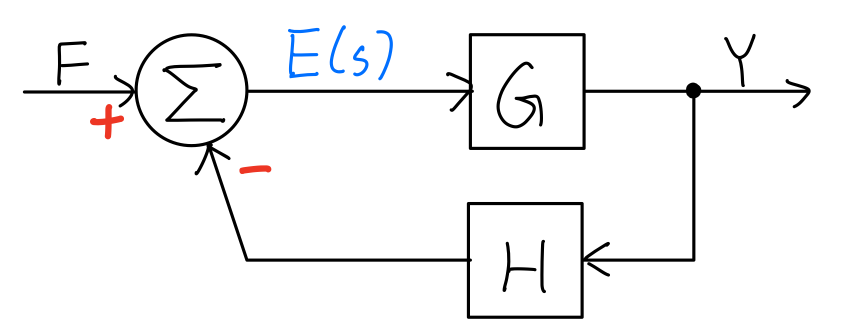
\includegraphics[width=0.5\linewidth]{figures/feedback.png}

    \blue{Canonical}\\
    \(
    \setlength{\jot}{0pt} 
    \begin{aligned}    
        F(s) &= \red{1} s^3 X + a_2s^2 X + a_1 sX + a_0 X\\      
        s^3 X &= F \red - a_2 s^2 X \red - a_1 sX \red - a_0 X         
    \end{aligned}
    \)\\
    \(b_3 s^3 X + b_2 s^2 X + b_1 sX + b_0 X = Y(s)\)

    % m < n for the state-space example!
    % here I use a first-degree denom for demonstration
    \(H = \frac{b_1s+b_0}{\red{1}s^3+a_2s^2+a_1s+a_0}\)\\     
    % note x1 x2 x3 back to front
    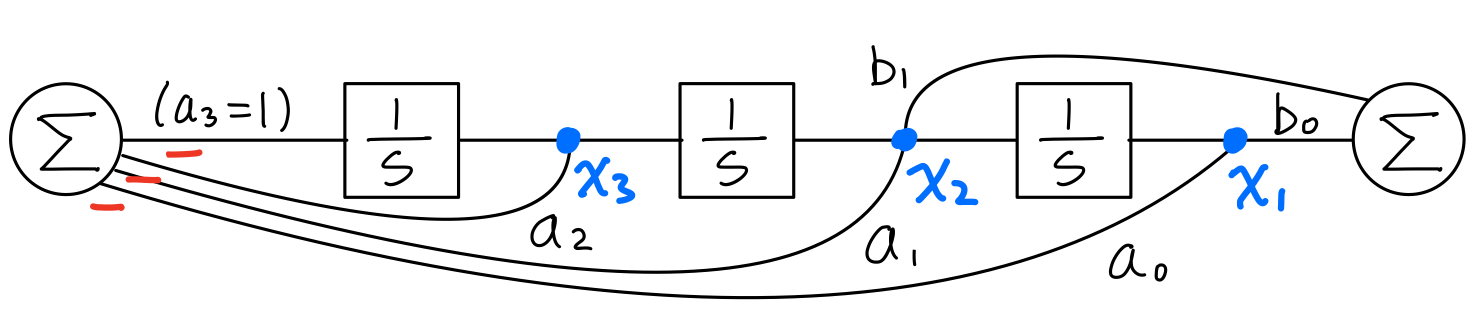
\includegraphics[width=\linewidth]{figures/canonical.png}
    \(
    \begin{bmatrix}
        \dot{x}_1\\
        \dot{x}_2\\
        \dot{x}_3\\
    \end{bmatrix}
    =
    \begin{bmatrix}
        0 & \red 1 & 0\\
        0 & 0 & \red 1\\
        -a_0 & -a_1 & -a_2
    \end{bmatrix}
    \begin{bmatrix}
        x_1\\
        x_2\\
        x_3
    \end{bmatrix}
    +
    \begin{bmatrix}
        0\\0\\\red{1}        % always 0 0 1
    \end{bmatrix}
    f
    \)\\

    \(y =
    \begin{bmatrix}
        b_0 & b_1 & 0      % b_0, b_1, ..., b_m, 0, ..., 0
    \end{bmatrix}
    \cdot \mathbf x
    \)

    % textbook p793 extra material
    % used a second degree example here to save space, sorry if it's confusing
    Second form: \(s^2 Y = s^2 b_2 F + s(-a_1 Y + b_1 F) + (-a_o Y + b_0 F)\)\\
        \hspace{1em} \(Y = b_2 F + \frac 1 s(-a_1 Y + b_1 F) + \frac 1 {s^2}(-a_o Y + b_0 F)\)\\
    Transpose $\mathbf A$, swap and trans $\mathbf b$, $\mathbf c$

\columnbreak
    % this is not that generalizable, compared to the other two
    \blue{Cascade} (made $P_3(s)$ constant here)\\
    \(H = \frac {P_1(s)}{s+\lambda_1} \cdot \frac{P_2(s)}{s+\lambda_2} \cdot \frac{k_3}{s+\lambda_3}\)\\
    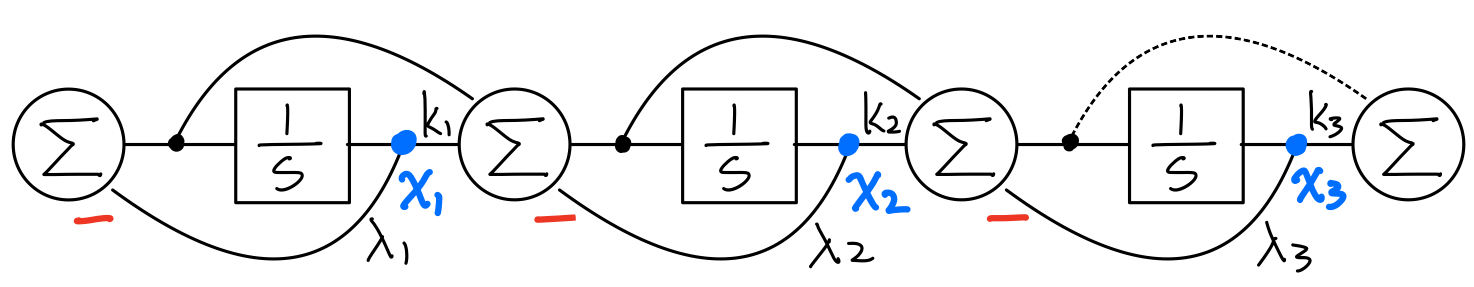
\includegraphics[width=\linewidth]{figures/cascade.png}
    \(
    \begin{bmatrix}
        \dot{x}_1\\
        \dot{x}_2\\
        \dot{x}_3\\
    \end{bmatrix}
    =
    \begin{bmatrix}
        \red{-\lambda_1} & 0 & 0\\
        .. & \red{-\lambda_2} & 0\\
        .. & .. & \red{-\lambda_3}\\ 
    \end{bmatrix}
    \begin{bmatrix}
        x_1\\
        x_2\\
        x_3
    \end{bmatrix}
    +
    \begin{bmatrix}
        1\\..\\..         % always 1 x x
    \end{bmatrix}
    f
    \)\\

    \(y =
    \begin{bmatrix}
        0 & 0 & k_3       % always x x 1
    \end{bmatrix}
    \cdot \mathbf x
    \)

    \blue{Parallel}\\
    \(H = \frac{k_1}{s+\lambda_1} + \frac{k_2}{s+\lambda_2} + \frac{k_3}{s+\lambda_3}\)\\
    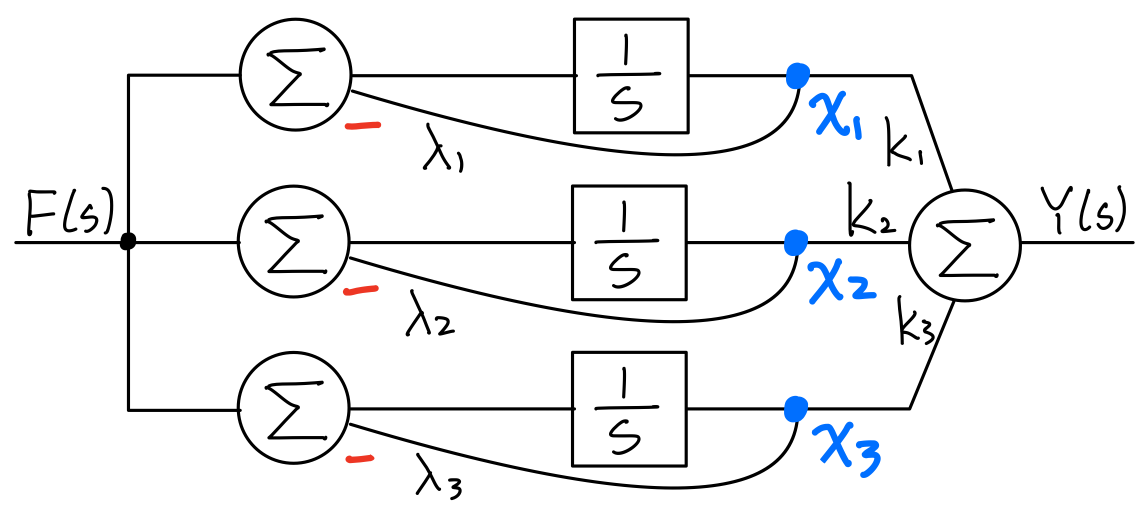
\includegraphics[width=0.75\linewidth]{figures/parallel.png}
    \(
    \begin{bmatrix}
        \dot{x}_1\\
        \dot{x}_2\\
        \dot{x}_3\\
    \end{bmatrix}
    =
    \begin{bmatrix}
        \red{-\lambda_1} & 0 & 0\\
        0 & \red{-\lambda_2} & 0\\
        0 & 0 & \red{-\lambda_3}\\ 
    \end{bmatrix}
    \begin{bmatrix}
        x_1\\
        x_2\\
        x_3
    \end{bmatrix}
    +
    \begin{bmatrix}
        1\\1\\1         % always 1 1 1
    \end{bmatrix}
    f
    \)\\

    \(y =
    \begin{bmatrix}
        k_1 & k_2 & k_3       % k_1, ..., k_n
    \end{bmatrix}
    \cdot \mathbf x
    \)

    \blue{(same pole)}                   
    \(H = \frac{a_0}{(s-\lambda)^{\red 2}} + \frac{a_1}{s-\lambda} + \frac{k_1}{s-\alpha_1}\)     
    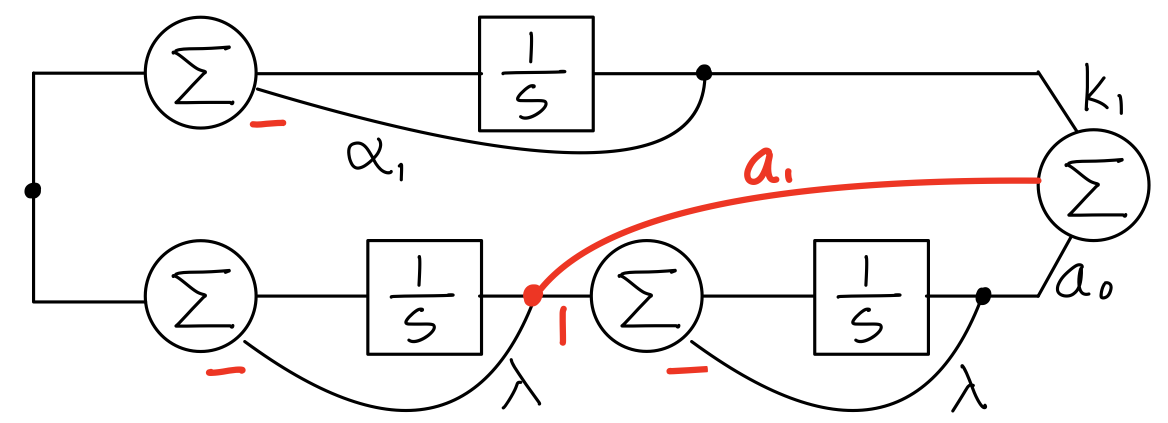
\includegraphics[width=0.7\linewidth]{figures/multipole.png}

\columnbreak
\subsubsection*{\blue{State Equations}}
    Def: \textit{state} of a sys at any time $t_0$ is the \textit{smallest} set of nums $\{x_i(t_0)\}$
        that is sufficient to detemrine sys behavior $\forall t > t_0$ 
        when input $f(t)$ is known for $t > t_0$\\
    Always \fbox{$\int$} output\\
    If $t_0 = 0$, initial condition


    \(\mathbf{\dot x} = \mathbf A \mathbf x + \mathbf b f\)\\
    \(y = \mathbf{c} \cdot \mathbf x\)\\
    \blue{MIMO}\\
    \(\mathbf{\dot x} = \mathbf A \mathbf x + \mathbf B \mathbf f\)\\
    \(\mathbf y = \mathbf C \mathbf x + \mathbf D \mathbf f\)

    \(
        \setlength{\jot}{0pt} % reduce the space between lines
        \begin{aligned}
            s \mathbf X(s) - \mathbf x(0) &= \mathbf A \mathbf X(s) + \mathbf B \mathbf F(s) \\
            (s \mathbf I - \mathbf A) \mathbf X(s) &= \mathbf x(0) + \mathbf B \mathbf F(s) \\
            \mathbf X(s) &= (s \mathbf I - \mathbf A)^{-1} \mathbf x(0) + (s \mathbf I - \mathbf A)^{-1} \mathbf B \mathbf F(s)\\
            \mathbf x(t) &= \mathbf x_{zi}(t) + \mathbf x_{zs}(t)
        \end{aligned}
    \)
\subsubsection*{\blue{LTI Freq Response}}
    \(H(\o) = H(s)|_{s = j\o} = \frac{P(s)}{Q(s)}\)     % first H is F, second is L

    Ideal delay: \(|H| = 1, \angle H(\o) = -\o T\)\\      % comes from exp(j..)
    Ideal diff: \(|H(\o)| = \red{|} \o \red{|}, \angle H(\o) = \pm\frac {\pi} 2\)\\
    Ideal int: \(|H(\o)| = \frac 1 {|\o|}\), \(\angle H(\o) = \mp \frac{\pi} 2\)
    % symmetry for -omega

    \(f(t) = \blue C = Ce^{0t}\)\\
    \(y(t) = H(0) C\)

    \(f(t) = \blue{e^{st}}\) \hfill everlasting\\
    \(y(t) = h(t) * e^{st} = e^{st} \int h(\tau) e^{-s\tau} d\tau \equiv H(s) e^{st}\)

    \(f(t) = e^{\red{j} \o_0 t}\, \red{u(t)}\)\\ 
    \(Y_{\red{zs}}(s) = F(s) H(s)\)\\     
    \(\hspace{3em}= \frac 1 {s - j\o_0} \frac{P(s)}{(s-\lambda_1)...(s-\lambda_n)}\)\\
    \(\hspace{3em}= \frac{H(s)|_{s=j\o_0}}{s-j\o_0} + \frac{k_1}{s-\lambda_1} + ...\)\\
    \(y_{\red{zs}}(t) = H(\o_0)  e^{j\o_0 t} \, \red{u(t)} + \sum_i k_i e^{\lambda_i t} \, \red{u(t)}\)

    $y_{ss}(t)$ scaled input\\
    $y_{tr}(t)$ decays for stable sys

    \(f(t) = \cos(\o_0 t + \theta) \, \red{u(t)}\)\\
    \(y_{\red{ss}}(t) = |H(\o_0)| \cos(\o_0 t + \theta + \angle H(\o_0)) \, \red{u(t)}\)

\subsubsection*{\blue{Pole Zero}}
    \(H(j\o) = b_n \frac{(j\o-z_1)..(j\o-z_n)}{(j\o-p_1)..(j\o-p_n)}\)\\\
    \(\hspace{2.75em} \equiv b_n \frac{(r_1 e^{j\phi_1})...(r_n e^{j\phi_n})}{(d_1 e^{j\theta_1})... (d_n e^{j\theta_n})}\)\\
    \(|H(\o)| = b_n \frac{r_1 ... r_n}{d_1 ... d_n}\)\\
    \(\angle H(\o) = (\phi_1 + .. + \phi_n) - (\theta_1 + .. + \theta_n)\)          % symmetry here!
    % give a graphical example
    % example of z = -1, p = -2 may be useful

    Vector from p/z to $j\o$\\
    Pole enhances gain; Zero suppresses
\end{multicols}
\end{landscape}
\end{document}
